%%%%%%%%%%%%%%%%%%%%%%%%%%%%%%%%%%%%%%%%%
% Beamer Presentation
% LaTeX Template
% Version 1.0 (10/11/12)
%
% This template has been downloaded from:
% http://www.LaTeXTemplates.com
%
% License:
% CC BY-NC-SA 3.0 (http://creativecommons.org/licenses/by-nc-sa/3.0/)
%
%%%%%%%%%%%%%%%%%%%%%%%%%%%%%%%%%%%%%%%%%

%----------------------------------------------------------------------------------------
%	PACKAGES AND THEMES
%----------------------------------------------------------------------------------------

\documentclass[UTF8,aspectratio=169,14pt]{ctexbeamer}

\usepackage{hyperref}
\hypersetup{
	colorlinks=true,
	linkcolor=red,
	anchorcolor=blue,
	citecolor=green
}

\mode<presentation> {
	
	% The Beamer class comes with a number of default slide themes
	% which change the colors and layouts of slides. Below this is a list
	% of all the themes, uncomment each in turn to see what they look like.
	
	%\usetheme{default}
	%\usetheme{AnnArbor}
	%\usetheme{Antibes}
	%\usetheme{Bergen}
	%\usetheme{Berkeley}
	%\usetheme{Berlin}
	%\usetheme{Boadilla}
	%\usetheme{CambridgeUS}
	%\usetheme{Copenhagen}
	%\usetheme{Darmstadt}
	%\usetheme{Dresden}
	%\usetheme{Frankfurt}
	%\usetheme{Goettingen}
	%\usetheme{Hannover}
	%\usetheme{Ilmenau}
	%\usetheme{JuanLesPins}
	%\usetheme{Luebeck}
	\usetheme{Madrid}
	%\usetheme{Malmoe}
	%\usetheme{Marburg}
	%\usetheme{Montpellier}
	%\usetheme{PaloAlto}
	%\usetheme{Pittsburgh}
	%\usetheme{Rochester}
	%\usetheme{Singapore}
	%\usetheme{Szeged}
	%\usetheme{Warsaw}
	
	% As well as themes, the Beamer class has a number of color themes
	% for any slide theme. Uncomment each of these in turn to see how it
	% changes the colors of your current slide theme.
	
	%\usecolortheme{albatross}
	%\usecolortheme{beaver}
	%\usecolortheme{beetle}
	%\usecolortheme{crane}
	%\usecolortheme{dolphin}
	%\usecolortheme{dove}
	%\usecolortheme{fly}
	%\usecolortheme{lily}
	%\usecolortheme{orchid}
	%\usecolortheme{rose}
	%\usecolortheme{seagull}
	%\usecolortheme{seahorse}
	%\usecolortheme{whale}
	%\usecolortheme{wolverine}
	
	%\setbeamertemplate{footline} % To remove the footer line in all slides uncomment this line
	%\setbeamertemplate{footline}[page number] % To replace the footer line in all slides with a simple slide count uncomment this line
	
	%\setbeamertemplate{navigation symbols}{} % To remove the navigation symbols from the bottom of all slides uncomment this line
}

\usepackage{graphicx} % Allows including images
\graphicspath{{./figs/}}
\usepackage{booktabs} % Allows the use of \toprule, \midrule and \bottomrule in tables
\usepackage{longtable}
\usepackage{listings}
\usepackage{xcolor}
\lstset{numbers=left, %设置行号位置
	numberstyle=\tiny, %设置行号大小
	keywordstyle=\color{blue}, %设置关键字颜色
	commentstyle=\color[cmyk]{1,0,1,0}, %设置注释颜色
	frame=single, %设置边框格式
	escapeinside=``, %逃逸字符(1左面的键),用于显示中文
	%breaklines, %自动折行
	extendedchars=false, %解决代码跨页时,章节标题,页眉等汉字不显示的问题
	xleftmargin=2em,xrightmargin=2em, aboveskip=1em, %设置边距
	tabsize=4, %设置tab空格数
	showspaces=false %不显示空格
}
% Fonts
% \usepackage{libertine}
% \setmonofont{Courier}
\setCJKsansfont[ItalicFont=Noto Serif CJK SC Black, BoldFont=Noto Sans CJK SC Black]{Noto Sans CJK SC}


%----------------------------------------------------------------------------------------
%	TITLE PAGE
%----------------------------------------------------------------------------------------

\title[第16讲]{第十六讲 :进程通信} % The short title appears at the bottom of every slide, the full title is only on the title page
\subtitle{第3节:Linux信号机制}
\author{向勇、陈渝、李国良} % Your name
\institute[清华大学] % Your institution as it will appear on the bottom of every slide, may be shorthand to save space
{
	清华大学计算机系 \\ % Your institution for the title page
	\medskip
	\textit{xyong,yuchen,liguoliang@tsinghua.edu.cn} % Your email address
}
\date{\today} % Date, can be changed to a custom date

\begin{document}

\begin{frame}
\titlepage % Print the title page as the first slide
\end{frame}

%----------------------------------------------
\begin{frame}
\frametitle{提纲} % Table of contents slide, comment this block out to remove it
\tableofcontents % Throughout your presentation, if you choose to use \section{} and \subsection{} commands, these will automatically be printed on this slide as an overview of your presentation

\pause

Ref: 
\href{http://ermak.cs.nstu.ru/understanding.linux.kernel.pdf }{Understanding the Linux Kernel}

\href{https://compas.cs.stonybrook.edu/~nhonarmand/courses/fa14/cse506.2/slides/ipc.pdf}{Signals and Inter-Process Communication}
\end{frame}
%----------------------------------------------
%%	PRESENTATION SLIDES
%----------------------------------------------
\section{第3节:Linux信号机制} % Sections can be created in order to organize your presentation into discrete blocks, all sections and subsections are automatically printed in the table of contents as an overview of the talk
%----------------------------------------------
\subsection{Signal Model} % A subsection can be created just before a set of slides with a common theme to further break down your presentation into chunks
%----------------------------------------------
\begin{frame}[fragile]
    \frametitle{信号(Signal)概念}

    \begin{itemize}
        \item 信号
        \begin{itemize}
            \item 进程间的软件中断通知和处理机制
            \item 如:SIGKILL, SIGSTOP, SIGCONT等
        \end{itemize} \pause

        \item 信号的接收处理
        \begin{itemize}
            \item 捕获(catch):执行进程指定的信号处理函数被调用
            \item 忽略(Ignore):执行操作系统指定的缺省处理
            \begin{itemize}
                \item 例如:进程终止、进程挂起等
            \end{itemize}
            \item 屏蔽(Mask):禁止进程接收和处理信号
            \begin{itemize}
                \item 可能是暂时的(当处理同样类型的信号)
            \end{itemize}
        \end{itemize} \pause

        \item 不足
        \begin{itemize}
            \item 传送的信息量小,只有一个信号类型
        \end{itemize}
    \end{itemize}

\end{frame}
%------------------------------------------------
\begin{frame}[fragile]
    \frametitle{信号的工作原理}

    \begin{figure}
        \centering
        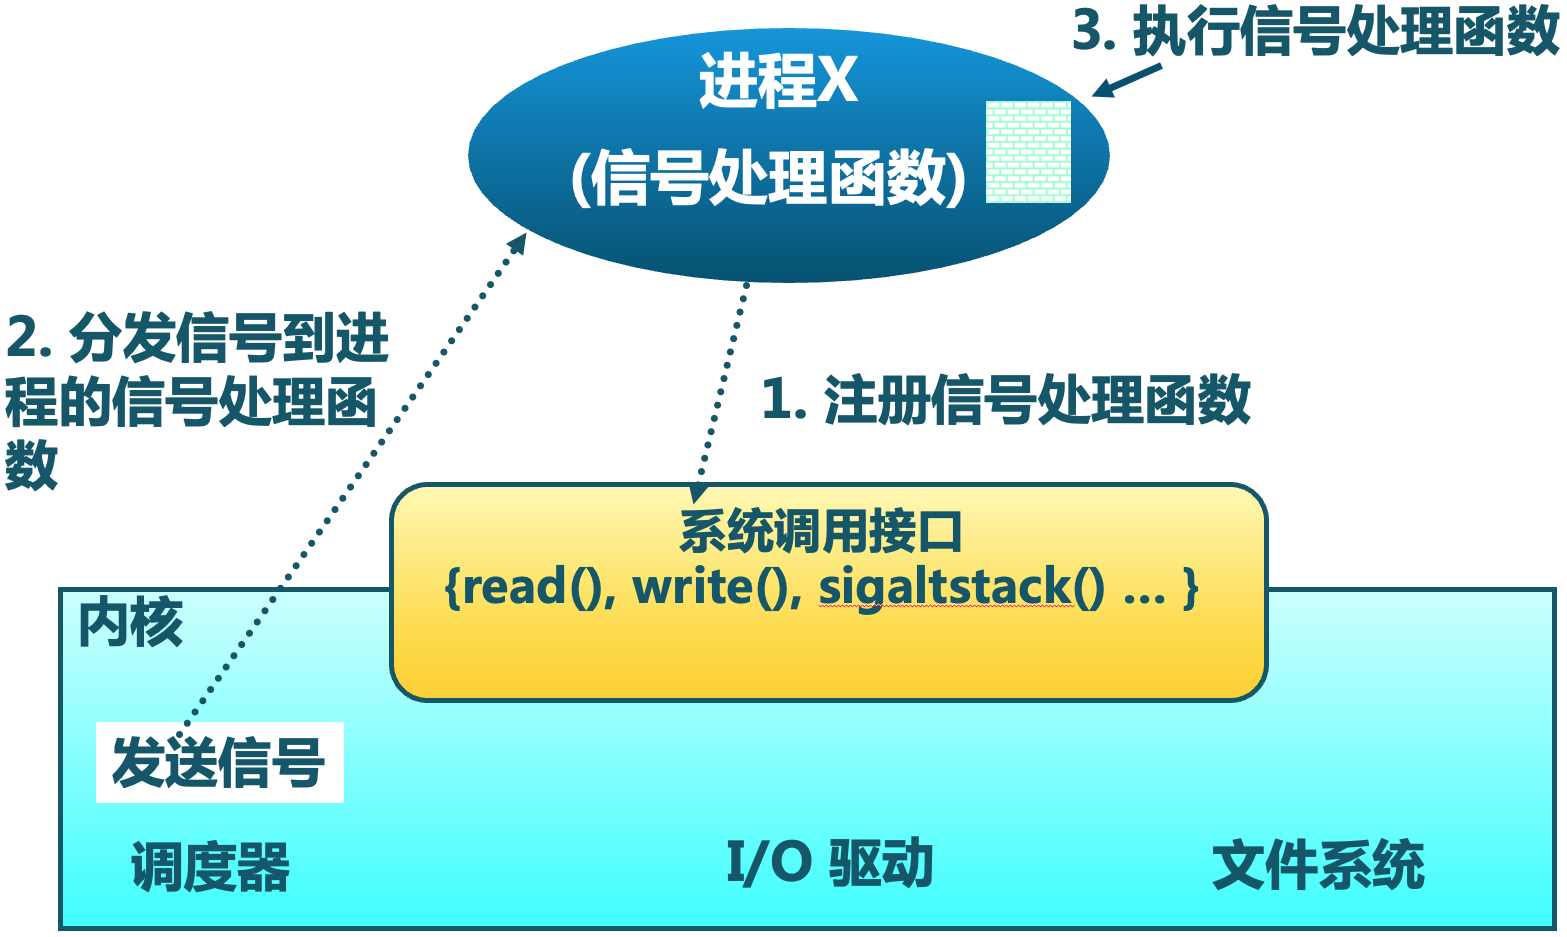
\includegraphics[width=0.8\linewidth]{figs/signal-method.png}
        % \caption{signal-method}
    \end{figure}

\end{frame}
%------------------------------------------------
\begin{frame}[fragile]
    \frametitle{Signal Model}
%    \framesubtitle{xxxx}
    \begin{itemize}
        \item Application registers handlers with \href{https://man7.org/linux/man-pages/man2/signal.2.html}{signal()} or \href{https://www.man7.org/linux/man-pages/man2/sigaction.2.html}{sigaction()} \pause
        \item Send signals with \href{https://man7.org/linux/man-pages/man2/kill.2.html}{kill()} and friends
        \begin{itemize}
            \item Or raised by hardware exception handlers in kernel
        \end{itemize} \pause
        \item Signal delivery jumps to signal handler
        \begin{itemize}
            \item Irregular control flow, similar to an interrupt
        \end{itemize}
    \end{itemize}
\end{frame}
%----------------------------------------------
% ### Signal Model
% #### Signal Model
% Ref: 20200410-09-ipc.pdf-Page:6
% 
%  * Application registers handlers with signal() or sigaction()
%  * Send signals with kill() and friends
%      * Or raised by hardware exception handlers in kernel
%  * Signal delivery jumps to signal handler
%      * Irregular control flow, similar to an interrupt
% 
%----------------------------------------------
\begin{frame}[fragile]
    \frametitle{信号使用\href{https://stackoverflow.com/questions/4217037/catch-ctrl-c-in-c}{示例}}
\tiny
\begin{semiverbatim}
\ #include <stdio.h>
\ #include <signal.h>
\ #include <stdlib.h>
\ void sigproc()
\ \{       
\     signal(SIGINT, sigproc);   /* NOTE some versions of UNIX will reset 
\                 * signal to default after each call. So for 
\                 * portability reset signal each time */
\     printf("you have pressed ctrl-c - disabled \\n");
\ \}
\ void quitproc()
\ \{        
\     printf("ctrl-\\\\ pressed to quit\\n");   /* this is “ctrl” \& “\\” */
\     exit(0); /* normal exit status */
\ \}
\ int main()
\ \{ 
\     signal(SIGINT, sigproc);    /* DEFAULT ACTION: term */
\     signal(SIGQUIT, quitproc);  /* DEFAULT ACTION: term */
\     printf("ctrl-c disabled use ctrl-\\\\ to quit\\n");
\     for(;;);
\ \}
\end{semiverbatim}

\end{frame}
%------------------------------------------------
\subsection{Signal Handler Control Flow} % A subsection can be created just before a set of slides with a common theme to further break down your presentation into chunks
%----------------------------------------------
\begin{frame}[fragile]
    \frametitle{Signal Handler Control Flow}
%    \framesubtitle{xxxx}
    \begin{figure}
	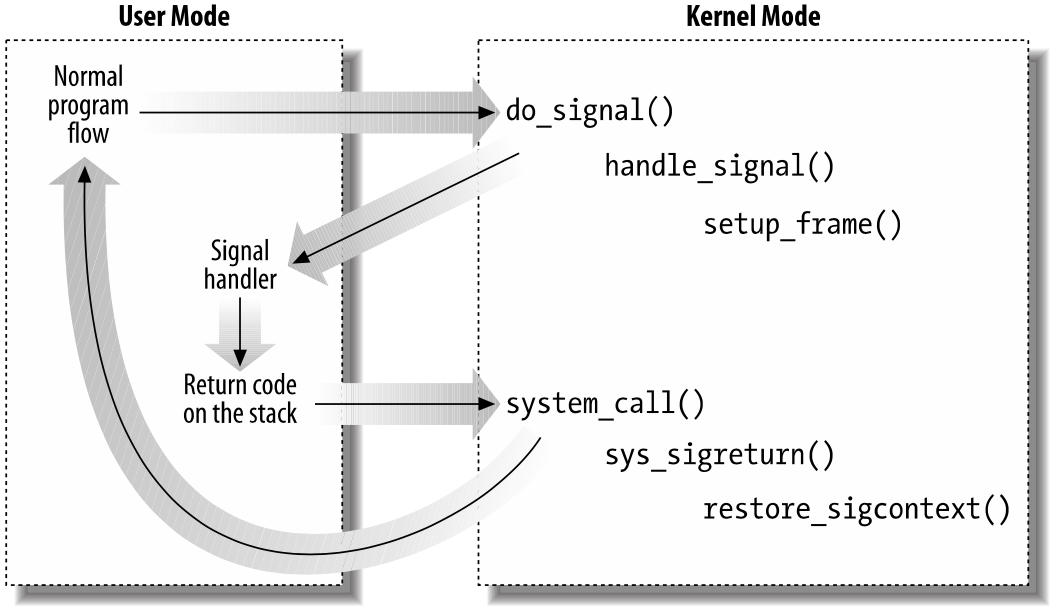
\includegraphics[width=0.8\linewidth]{figs/signal-control-flow.png}
%	\caption{xxxx}
	\end{figure}
\end{frame}
%----------------------------------------------
% ### Signal Handler Control Flow
% #### Signal Handler Control Flow
% Ref: 20200410-09-ipc.pdf-Page:9
% 
% ![signal-control-flow](figs/signal-control-flow.png)
% 
%----------------------------------------------
\begin{frame}[fragile]
    \frametitle{Alternate Stacks}
%    \framesubtitle{xxxx}
    \begin{itemize}
        \item Signal handlers can execute on a different stack than program execution.
        \begin{itemize}
            \item Set with \href{https://linux.die.net/man/3/sigaltstack}{sigaltstack()} system call
        \end{itemize} \pause
        \item Like an interrupt handler, kernel pushes register state on interrupt stack
        \begin{itemize}
            \item Return to kernel with \href{https://man7.org/linux/man-pages/man2/sigreturn.2.html}{sigreturn()} system call
            \item App can change its own on-stack register state!
        \end{itemize}
    \end{itemize}
\end{frame}
%----------------------------------------------
% #### Alternate Stacks
% Ref: 20200410-09-ipc.pdf-Page:10
% 
%  * Signal handlers can execute on a different stack than program execution.
%    * Set with sigaltstack() system call
%  * Like an interrupt handler, kernel pushes register state on interrupt stack
%    * Return to kernel with sigreturn() system call
%    * App can change its own on-stack register state!
% 
%----------------------------------------------
\begin{frame}[fragile]
    \frametitle{Frame on the User Mode stack}
%    \framesubtitle{xxxx}
    \begin{columns}
    \begin{column}{0.5\textwidth}
        \begin{figure}
        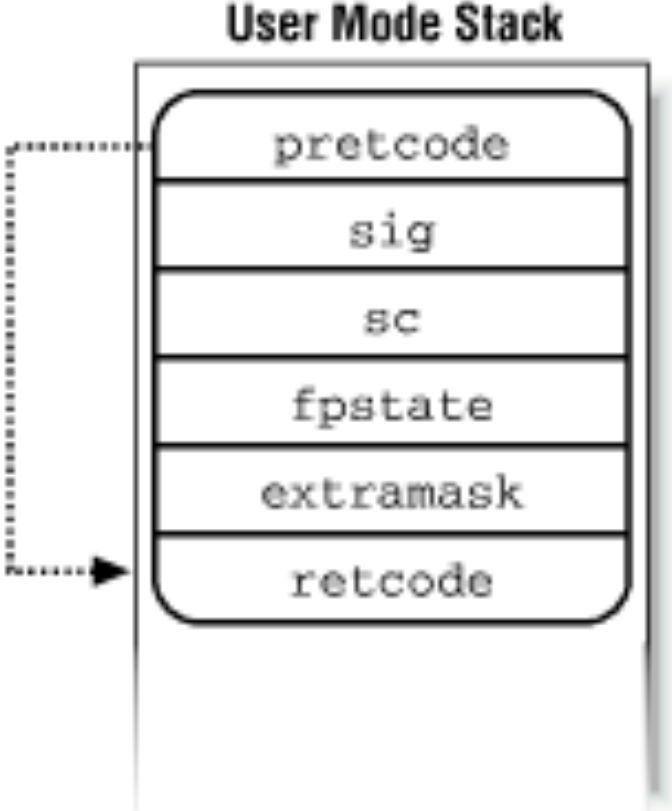
\includegraphics[width=0.8\linewidth]{figs/signal-stack-frame.png}
    %	\caption{xxxx}
        \end{figure}
	\end{column}
	\begin{column}{0.5\textwidth}
        \begin{itemize}
            \item pretcode: Return address of the signal handler function
            \item sig: Signal number \pause
            \item sc: Hardware context of the User Mode process
            \item fpstate: Floating point registers of the User Mode process
            \item extramask: Blocked real-time signals \pause
            \item retcode: Eight-byte code issuing a sigreturn() system call
        \end{itemize}
    \end{column}
	\end{columns}

\end{frame}
%----------------------------------------------
% #### Frame on the User Mode stack
% Ref: https://www.halolinux.us/kernel-reference/figure-103-frame-on-the-user-mode-stack.html
% 
% ![signal-stack-frame](figs/signal-stack-frame.png)
% 
%  * pretcode: Return address of the signal handler function;
%  * sig: The signal number; 
%  * sc: hardware context of the User Mode process
%  * fpstate: floating point registers of the User Mode process
%  * extramask: blocked real-time signals
%  * retcode: Eight-byte code issuing a sigreturn( ) system call;
% 
%----------------------------------------------
\begin{frame}[fragile]
    \frametitle{Signal trampoline \& sigreturn() syscall}
%    \framesubtitle{xxxx}
A small piece of assembly code to perform cleanup after handling the signal. \pause
    \begin{itemize}
        \item Signal trampoline code calls sigreturn(). \pause
        \item sigreturn() undoes everything that was done in order to invoke the signal handler
        \begin{itemize}
            \item Changing the process's signal mask, switching signal stacks
            \item switches stacks, and restores the process's context
            \item sigreturn() never returns
        \end{itemize} \pause
        \item Signal trampoline code lives either in the vDSO or in the C library.
        \begin{itemize}
            \item vDSO (virtual dynamic shared object): a small shared library that the kernel automatically maps into the address space of all user-space applications.
        \end{itemize}
    \end{itemize}
\end{frame}
%----------------------------------------------
% #### Signal trampoline & sigreturn() syscall
% Ref: https://www.netbsd.org/docs/internals/en/chap-processes.html#signal
% 
% a small piece of assembly code to perform cleanup after handling the signal.
% 
% The signal trampoline code in turn calls sigreturn().
% This sigreturn() call undoes everything that was done in order to invoke the signal handler.
% Changing the process's signal mask, switching signal stacks (see sigaltstack(2))
% switches stacks, and restores the process's context
% sigreturn() never returns
% the signal trampoline code lives either in the vDSO or in the C library.
% vDSO (virtual dynamic shared object): a small shared library that the kernel automatically maps into the address space of all user-space applications.
% 
%----------------------------------------------
\begin{frame}[fragile]
    \frametitle{Dealing With Asynchronous Signals In Multi Threaded Program}
%    \framesubtitle{xxxx}
The first available thread gets the signal. \pause
    \begin{itemize}
        \item Most handlers run on the thread's stack
        \item A handler can run on an alternate stack \pause
        \item Thread in the kernel does not run the handler until it goes to userspace.
    \end{itemize}
\end{frame}
%----------------------------------------------
% #### Dealing With Asynchronous Signals In Multi Threaded Program
% https://stackoverflow.com/questions/6949025/how-are-asynchronous-signal-handlers-executed-on-linux
% 
% The first available thread gets the signal
% Most handlers run on the thread's stack.
% A handler can run on an alternate stack
% the thread is running in the kernel does not run the handler until it goes to userspace.
% 
%----------------------------------------------
\subsection{Signal handlers} % A subsection can be created just before a set of slides with a common theme to further break down your presentation into chunks
%----------------------------------------------
\begin{frame}
\frametitle{提纲} % Table of contents slide, comment this block out to remove it
\tableofcontents % Throughout your presentation, if you choose to use \section{} and \subsection{} commands, these will automatically be printed on this slide as an overview of your presentation

\pause

Ref: 
\href{http://ermak.cs.nstu.ru/understanding.linux.kernel.pdf }{Understanding the Linux Kernel}

\href{https://compas.cs.stonybrook.edu/~nhonarmand/courses/fa14/cse506.2/slides/ipc.pdf}{Signals and Inter-Process Communication}
\end{frame}
%----------------------------------------------
\begin{frame}[fragile]
    \frametitle{Default Signal handlers}
%    \framesubtitle{xxxx}
    \begin{itemize}
        \item Signals have default handlers:
        \begin{itemize}
            \item Ignore, kill, suspend, continue, dump core
            \item These execute inside the kernel \pause
        \end{itemize}
        \item Installing a handler with signal()/sigaction() overrides the default
        \item A few (SIGKILL, SIGSTOP) cannot be overridden
    \end{itemize}
\end{frame}
%----------------------------------------------
% ### Signal handlers
% #### Default Signal handlers
% 
% Ref: 20200410-09-ipc.pdf-Page:11
% 
%  * Signals have default handlers:
%     * Ignore, kill, suspend, continue, dump core
%     * These execute inside the kernel
%  * Installing a handler with signal()/sigaction() overrides the default
%  * A few (SIGKILL, SIGSTOP) cannot be overridden
% 
%----------------------------------------------
\begin{frame}[fragile]
    \frametitle{Signal Delivery}
%    \framesubtitle{xxxx}
    \begin{itemize}
        \item Send a signal == mark a pending signal in the task
        \begin{itemize}
            \item And make runnable if blocked with TASK\_INTERRUPTIBLE flag
        \end{itemize} \pause
        \item Check pending signals on return from interrupt or syscall
        \begin{itemize}
            \item Deliver if pending
        \end{itemize}
    \end{itemize}
\end{frame}
%----------------------------------------------
% #### Signal Delivery
% Ref: 20200410-09-ipc.pdf-Page:12
%  * Kernel is lazy!
%     * Send a signal == mark a pending signal in the task
%        * And make runnable if blocked with TASK_INTERRUPTIBLE flag
%     * Check pending signals on return from interrupt or syscall
%        * Deliver if pending
% 
%----------------------------------------------
\begin{frame}[fragile]
    \frametitle{Nested Signals}
%    \framesubtitle{xxxx}
    \begin{itemize}
        \item sigaction() API lets you specify this in detail
        \begin{itemize}
            \item What signals are blocked (and delivered on sigreturn)
            \item Similar to disabling hardware interrupts
        \end{itemize} \pause
        \item Blocking system calls inside of a signal handler are only safe with careful use of sigaction()
    \end{itemize}
\end{frame}
%----------------------------------------------
% #### Nested Signals
% Ref: 20200410-09-ipc.pdf-Page: 17
% 
%  * sigaction() API lets you specify this in detail
%     * What signals are blocked (and delivered on sigreturn)
%     * Similar to disabling hardware interrupts
%  * Blocking system calls inside of a signal handler are only safe with careful use of sigaction()% 
%----------------------------------------------
\subsection{Language Exceptions} % A subsection can be created just before a set of slides with a common theme to further break down your presentation into chunks
%----------------------------------------------
\begin{frame}[fragile]
    \frametitle{\href{https://www.cs.york.ac.uk/rts/books/RTSbookThirdEdition/chap6.pdf}{C Exceptions}}

    \begin{itemize}
        \item C does not define any exception handling facilities
        \item This  clearly  limits  its  in  the  structured  programming  of  reliable systems
        \item Some form of exception handling mechanism by using the C macro facility
        \item Termination  model: Save  the status of a program's registers etc. on entry to an exception domain and then restore them if an exception occurs.
        \item The POSIX facilities of setjmp and longjmpcan be used for this purpose
    \end{itemize}

\end{frame}
%----------------------------------------------
\begin{frame}[fragile]
    \frametitle{Language Exceptions}
%    \framesubtitle{xxxx}
    \begin{itemize}
        \item Signals are the underlying mechanism for Exceptions and catch blocks \pause
        \item JVM or other runtime system sets signal handlers \pause
        \item Signal handler causes execution to jump to the catch block
    \end{itemize}
\end{frame}
%----------------------------------------------
% #### Language Exceptions
% Ref: 20200410-09-ipc.pdf-Page:8
% 
%  * Signals are the underlying mechanism for Exceptions and catch blocks
%  * JVM or other runtime system sets signal handlers
%  * Signal handler causes execution to jump to the catch block
%----------------------------------------------
\begin{frame}[fragile]
    \frametitle{\href{https://www.cs.york.ac.uk/rts/books/RTSbookThirdEdition/chap6.pdf}{C Exceptions}}

    \begin{itemize}
        \item C does not define any exception handling facilities
        \item This  clearly  limits  its  in  the  structured  programming  of  reliable systems
        \item Some form of exception handling mechanism by using the C macro facility
        \item Termination  model: Save  the status of a program's registers etc. on entry to an exception domain and then restore them if an exception occurs.
        \item The POSIX facilities of setjmp and longjmpcan be used for this purpose
    \end{itemize}

\end{frame}
%----------------------------------------------
\begin{frame}[fragile]
    \frametitle{\href{https://i0.wp.com/techvidvan.com/tutorials/wp-content/uploads/sites/2/2020/04/java-exception-hierarchy.jpg}{Java Exception Hierarchy}}
    \begin{figure}
    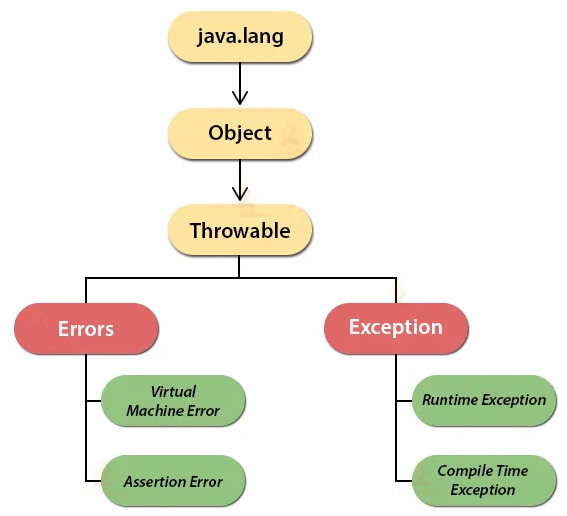
\includegraphics[width=0.5\linewidth]{figs/java-exception-hierarchy.png}
%   \caption{xxxx}
    \end{figure}

\end{frame}
%----------------------------------------------
\begin{frame}[fragile]
    \frametitle{\href{https://zhuanlan.zhihu.com/p/128953024}{Golang之信号处理(Signal)}}

    \begin{columns}[c] % The "c" option specifies centered vertical alignment while the "t" option is used for top vertical alignment

    \column{.45\textwidth} % Left column and width
        \begin{itemize}
            \item 注册SIGTERM信号的处理函数并在处理函数中做一些进程退出的准备,实现优雅退出。
            \item 信号的订阅是通过 channel实现的,每个os.Signal channel 都会收听自己相应的事件集。
        \end{itemize}

    \column{.5\textwidth} % Right column and width
        \begin{figure}
        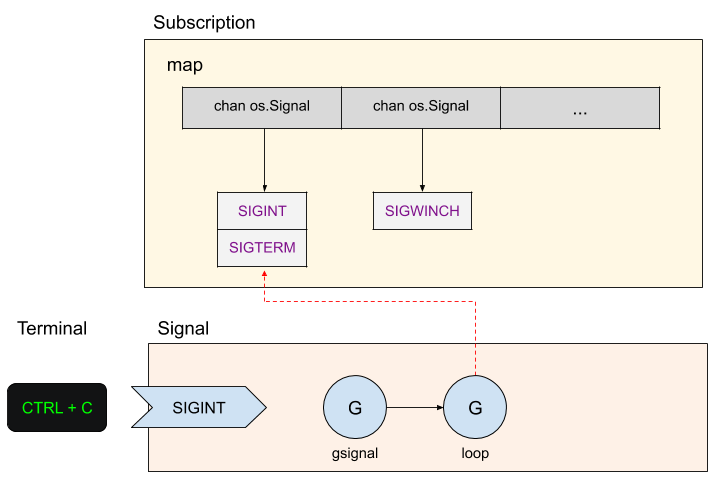
\includegraphics[width=1.0\linewidth]{figs/GO-signal.png}
    %   \caption{xxxx}
        \end{figure}

    \end{columns}

\end{frame}
%----------------------------------------------
\begin{frame}[fragile]
    \frametitle{\href{https://www.tutorialspoint.com/rust/rust_error_handling.htm}{Error Handling in Rust}}

    \begin{figure}
    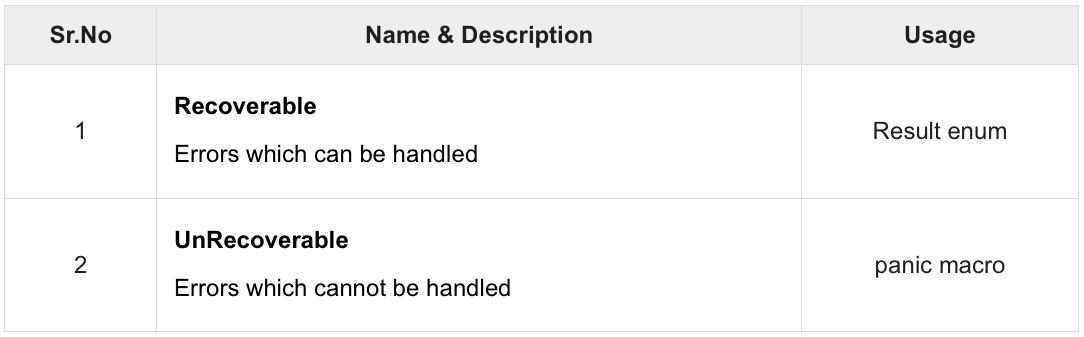
\includegraphics[width=1.0\linewidth]{figs/rust-error-handling.png}
%   \caption{xxxx}
    \end{figure}

\end{frame}
%----------------------------------------------

\end{document}
